\chapter{Appendix}

\section{Characterization of IDD feedtypes}

In Table.~\ref{tab:size-summary} and Table.~\ref{tab:inter-arr-time-summary}, we listed several quantiles of size and inter-arrival time of top five feedtypes.
In this appendix, we provide the histograms of size and inter-arrival time for the other 4 feedtypes (NGRID, NEXRAD2, NEXRAD3, FSL2).

\begin{figure}[htb!]
\centering
    \begin{subfigure}{0.5\linewidth}
        \centering
        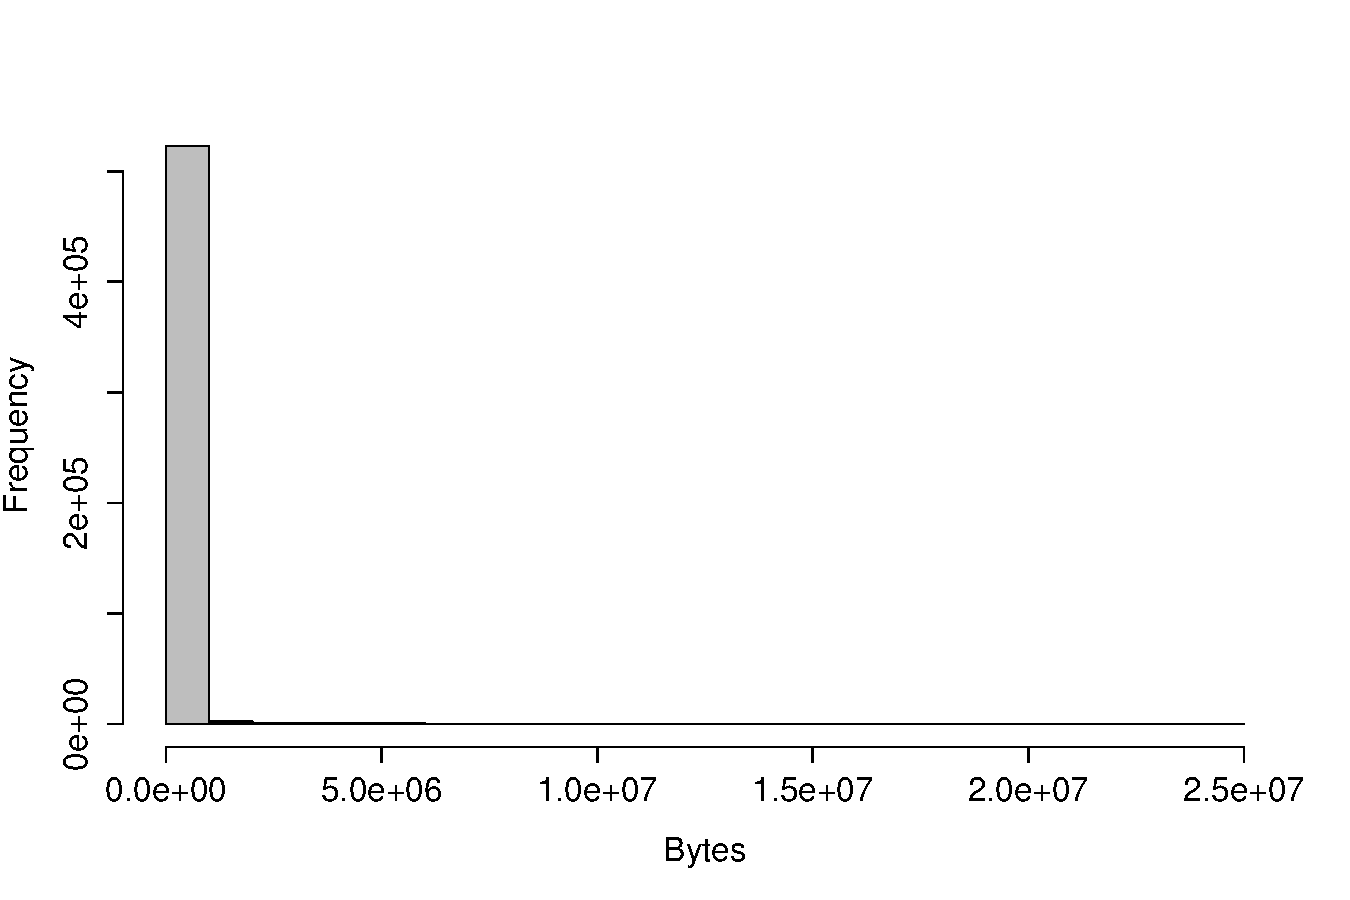
\includegraphics[width=2.2in]{figures/Size-hist-NGRID0602.pdf}
        \caption{Whole size range}
        \label{NGRID_Size_Whole}
    \end{subfigure}\hfill
    \begin{subfigure}{0.5\linewidth}
	\centering
    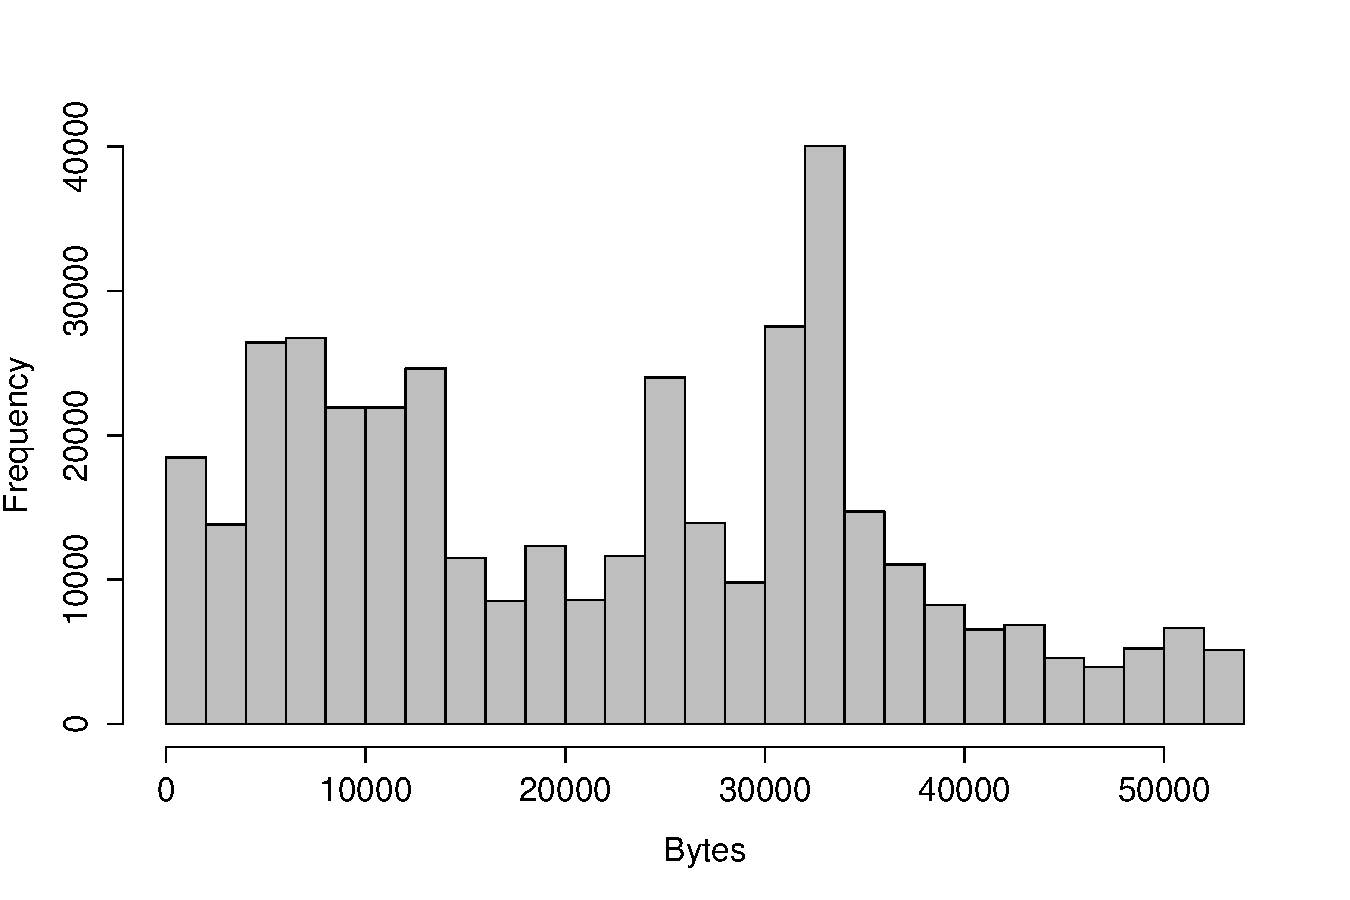
\includegraphics[width=2.2in]{figures/Size-hist-NGRID602-TOP75.pdf}
    %\includegraphics[width=3.5in]{figures/CONDUIT-size-75.eps}
        \caption{Top 75 percentile of size range}
        \label{NGRID_Size_75}
    \end{subfigure}\hfill
    \caption{NGRID feedtype, histograms of the size of the data products sent on June 02, 2014}
    \label{NGRID_Size}
\end{figure}

NGRID (NG) \cite{NGRID} feedtype is grided data from National Oceanic and Atospheric Administration (NOAA). Fig.~\ref{NGRID_Size} shows that almost 75\% data products are smaller than 50KB. Fig.~\ref{NG_time} shows that most of the inter-arrival time are less than 20ms.

\begin{figure}[htb!]
\centering
    \begin{subfigure}{0.5\linewidth}
        \centering
        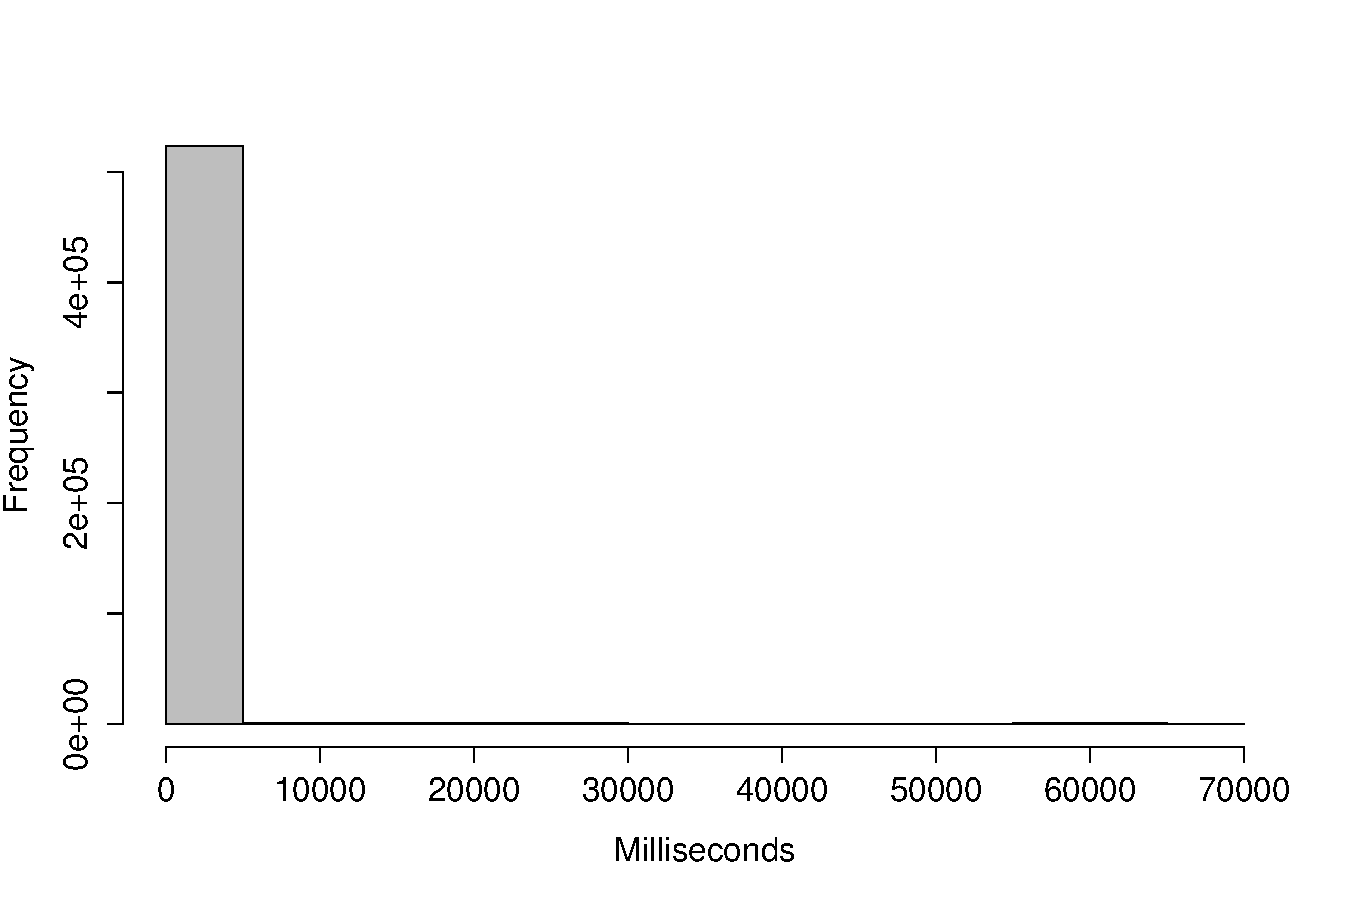
\includegraphics[width=2.2in]{figures/Inter-hist-NGRID0602.pdf}
        %\includegraphics[width=3.5in]{figures/CONDUIT_Size.eps}
        \caption{Whole inter-arrival time range}
        \label{NGRID_Inter_Whole}
    \end{subfigure}\hfill
    \begin{subfigure}{0.5\linewidth}
	\centering
    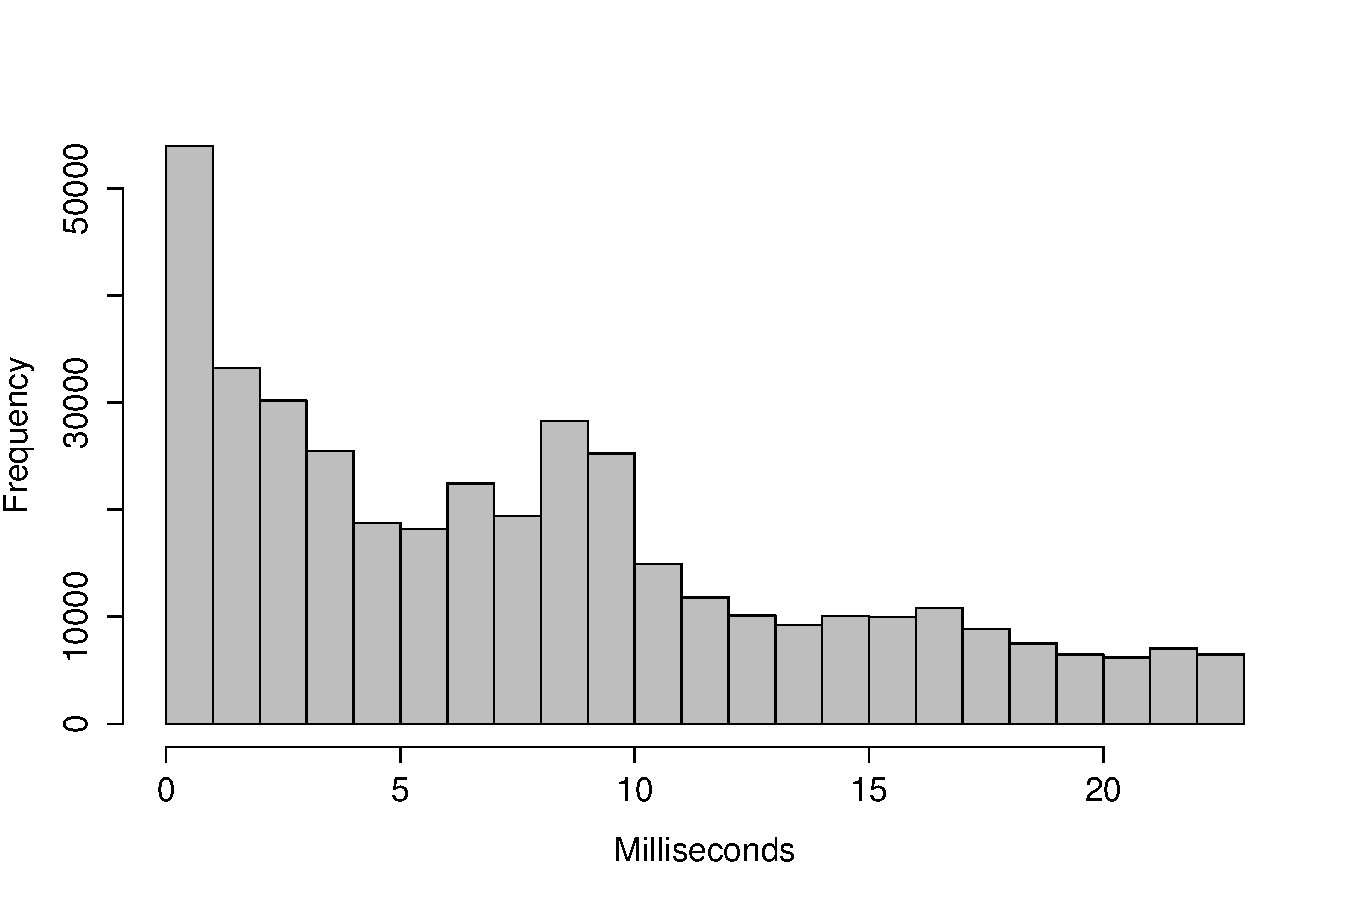
\includegraphics[width=2.2in]{figures/Inter-hist-NGRID0602-TOP75.pdf}
    %\includegraphics[width=3.5in]{figures/CONDUIT-size-75.eps}
        \caption{Top 75 percentile of inter-arrival time range}
        \label{NGRID_Inter_75}
    \end{subfigure}\hfill
    \caption{NGRID feedtype, histograms of inter-arrival time of data products sent on June 02, 2014, }
    \label{NG_time}
\end{figure}

%NEXRAD2-5
\begin{figure}[htb!]
\centering
    \begin{subfigure}{0.5\linewidth}
        \centering
        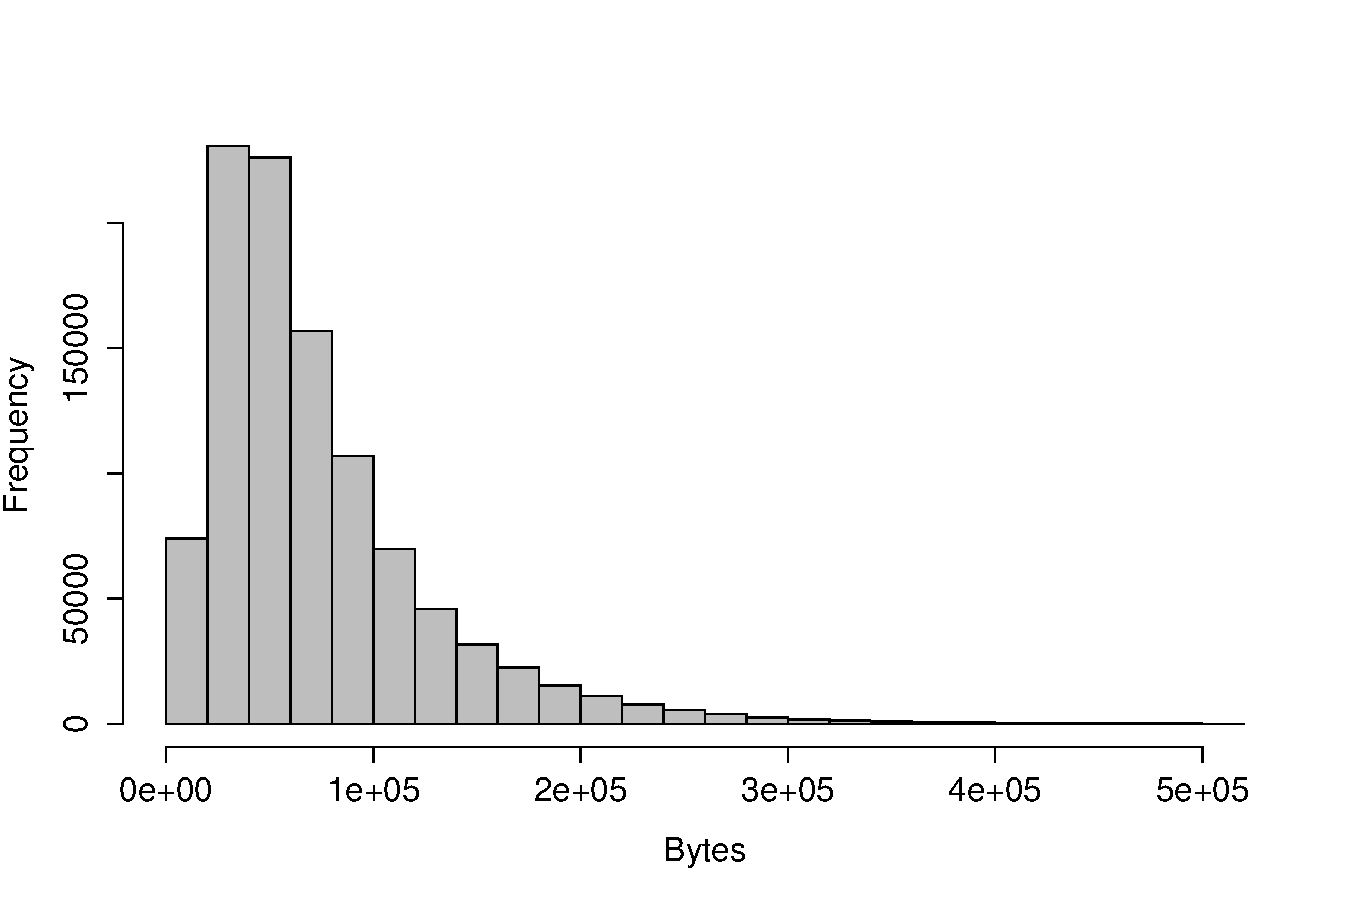
\includegraphics[width=2.2in]{figures/size-hist-NEXRAD20602.pdf}
        %\includegraphics[width=3.5in]{figures/CONDUIT_Size.eps}
        \caption{Whole size range }
        \label{NEXRAD2_Size_Whole}
    \end{subfigure}\hfill
    \begin{subfigure}{0.5\linewidth}
	\centering
    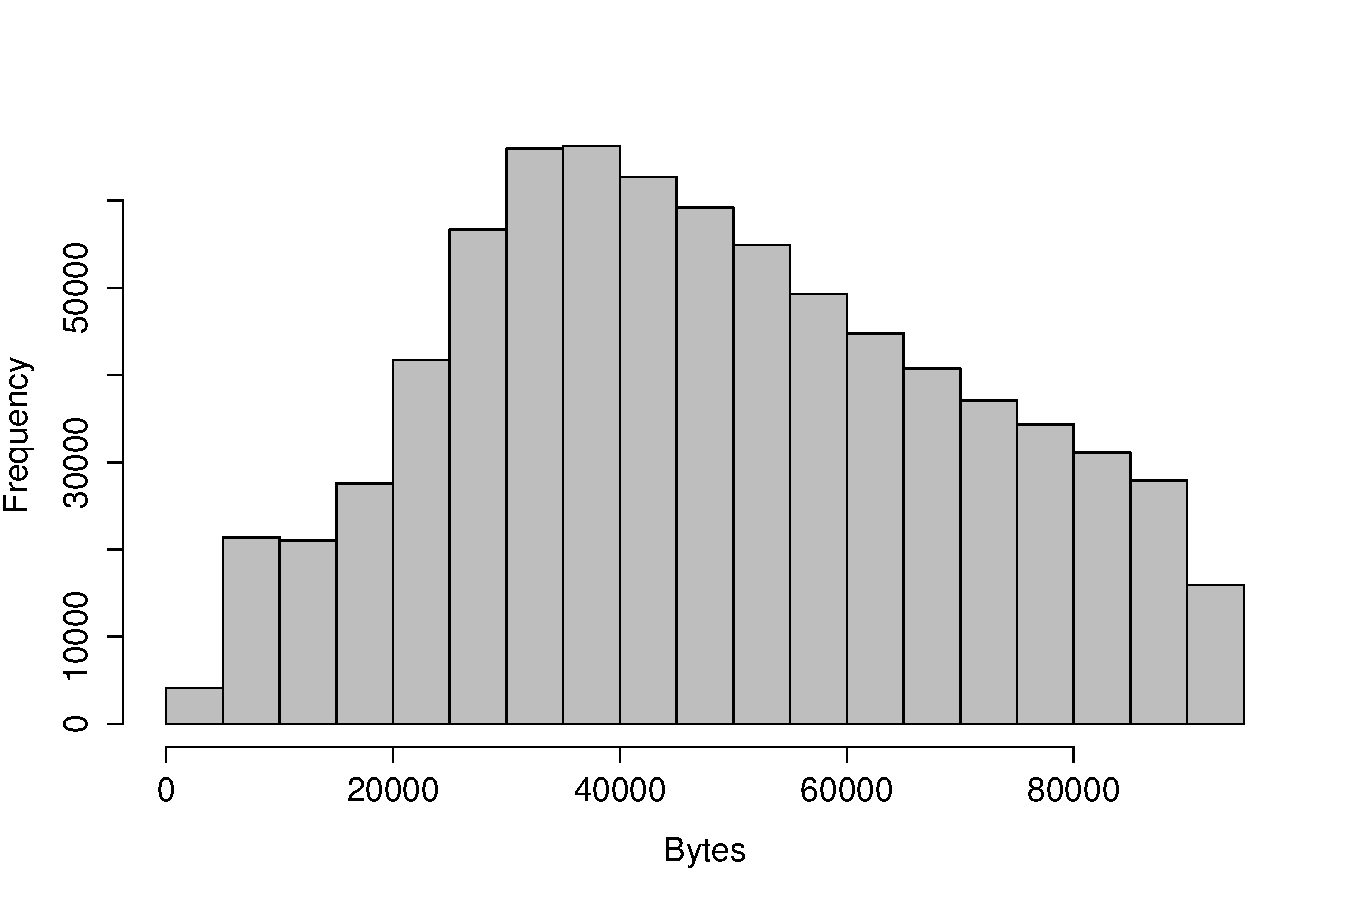
\includegraphics[width=2.2in]{figures/size-hist-NEXRAD20602-TOP75.pdf}
    %\includegraphics[width=3.5in]{figures/CONDUIT-size-75.eps}
        \caption{Top 75 percentile of size range}
        \label{NEXRAD2_Size_75}
    \end{subfigure}\hfill
    \caption{NEXRAD2 feedtype, histograms of size of data products sent on June 02, 2014}
    \label{NEXRAD2_Size}
\end{figure}

NEXRAD2 feedtype is NEXRAD level II radar data. Fig.~\ref{NEXRAD2_Size} shows the file size of this type of data is large. The top 75\% size histogram Fig.~\ref{NEXRAD2_Size_75} indicates that most of the size of data products are within 40KB.

\begin{figure}[htb!]
\centering
    \begin{subfigure}{0.5\linewidth}
        \centering
        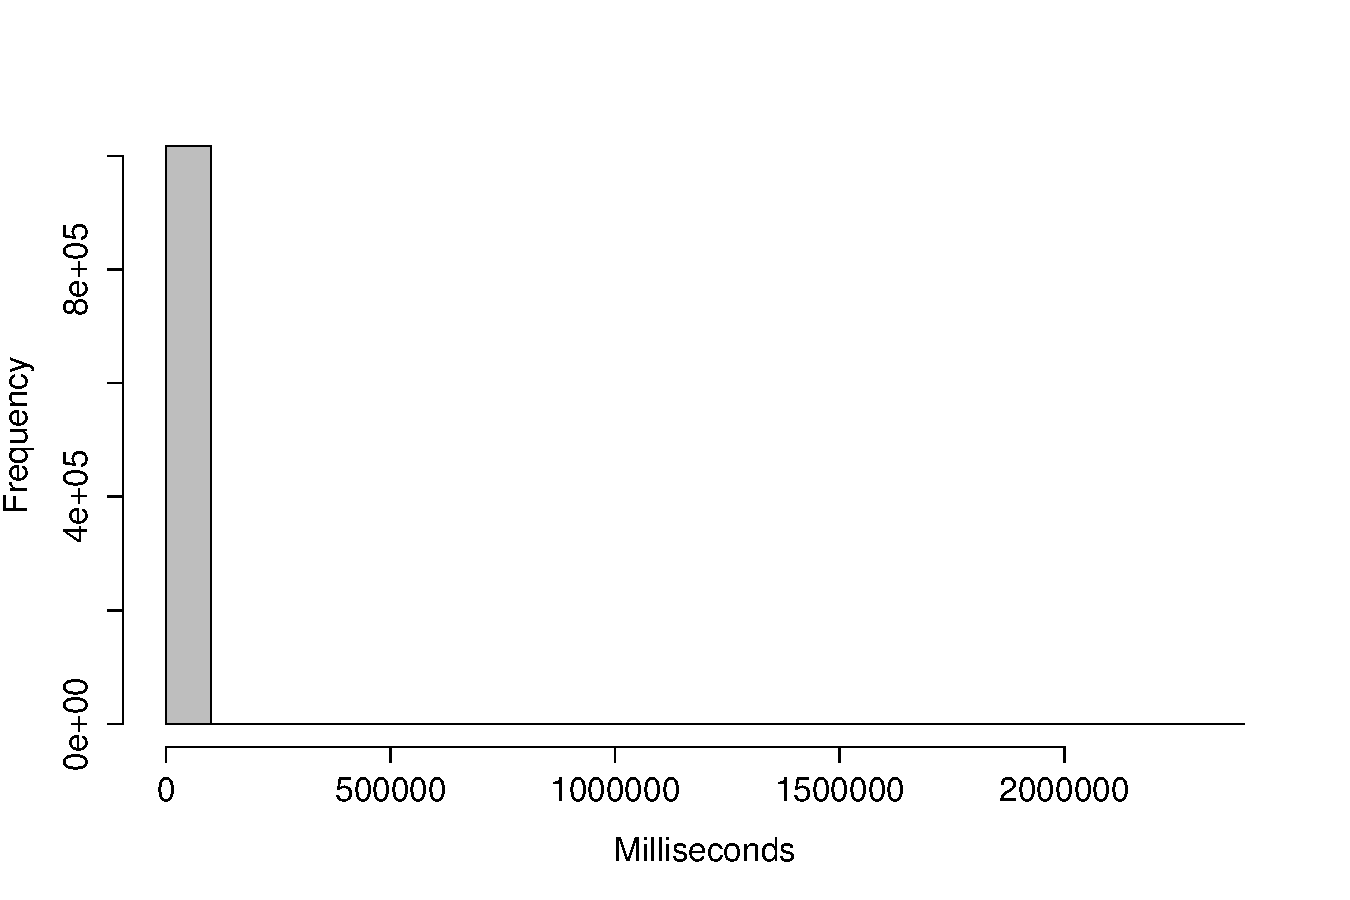
\includegraphics[width=2.2in]{figures/Inter-hist-NEXRAD20602.pdf}
        %\includegraphics[width=3.5in]{figures/CONDUIT_Size.eps}
        \caption{Whole inter-arrival time range}
        \label{NEXRAD2_Inter_Whole}
    \end{subfigure}\hfill
    \begin{subfigure}{0.5\linewidth}
	\centering
    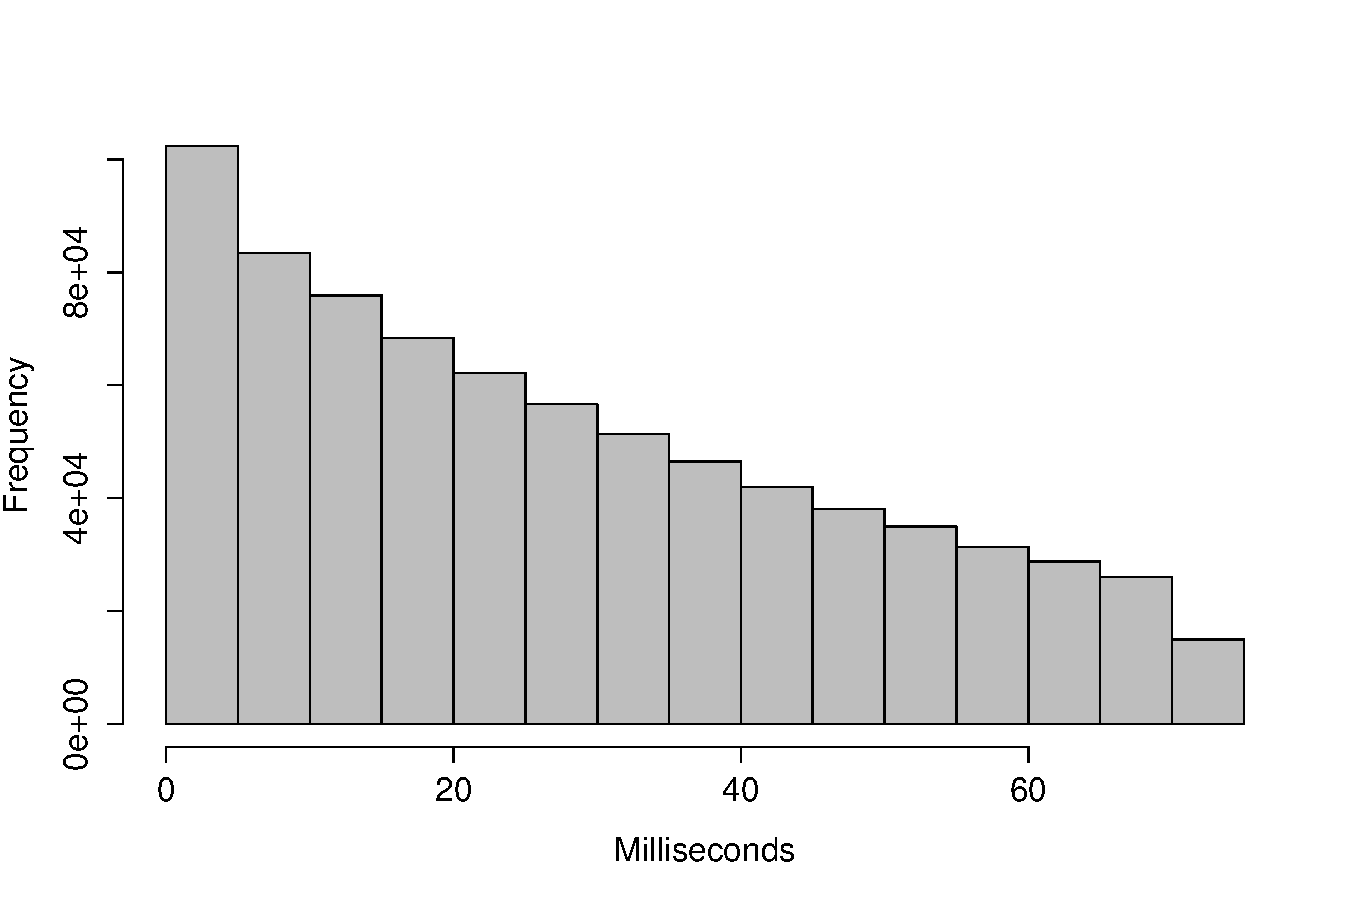
\includegraphics[width=2.2in]{figures/Inter-hist-NEXRAD20602-TOP75.pdf}
    %\includegraphics[width=3.5in]{figures/CONDUIT-size-75.eps}
        \caption{Top 75 percentile of inter-arrival time range}
        \label{NEXRAD2_Inter_75}
    \end{subfigure}\hfill
    \caption{NEXRAD2 feedtype, histograms of inter-arrival time of data products sent on June 02, 2014}
    \label{NEXRAD2_time}
\end{figure}

%NEXRAD3
\begin{figure}[htb!]
\centering
    \begin{subfigure}{0.5\linewidth}
        \centering
        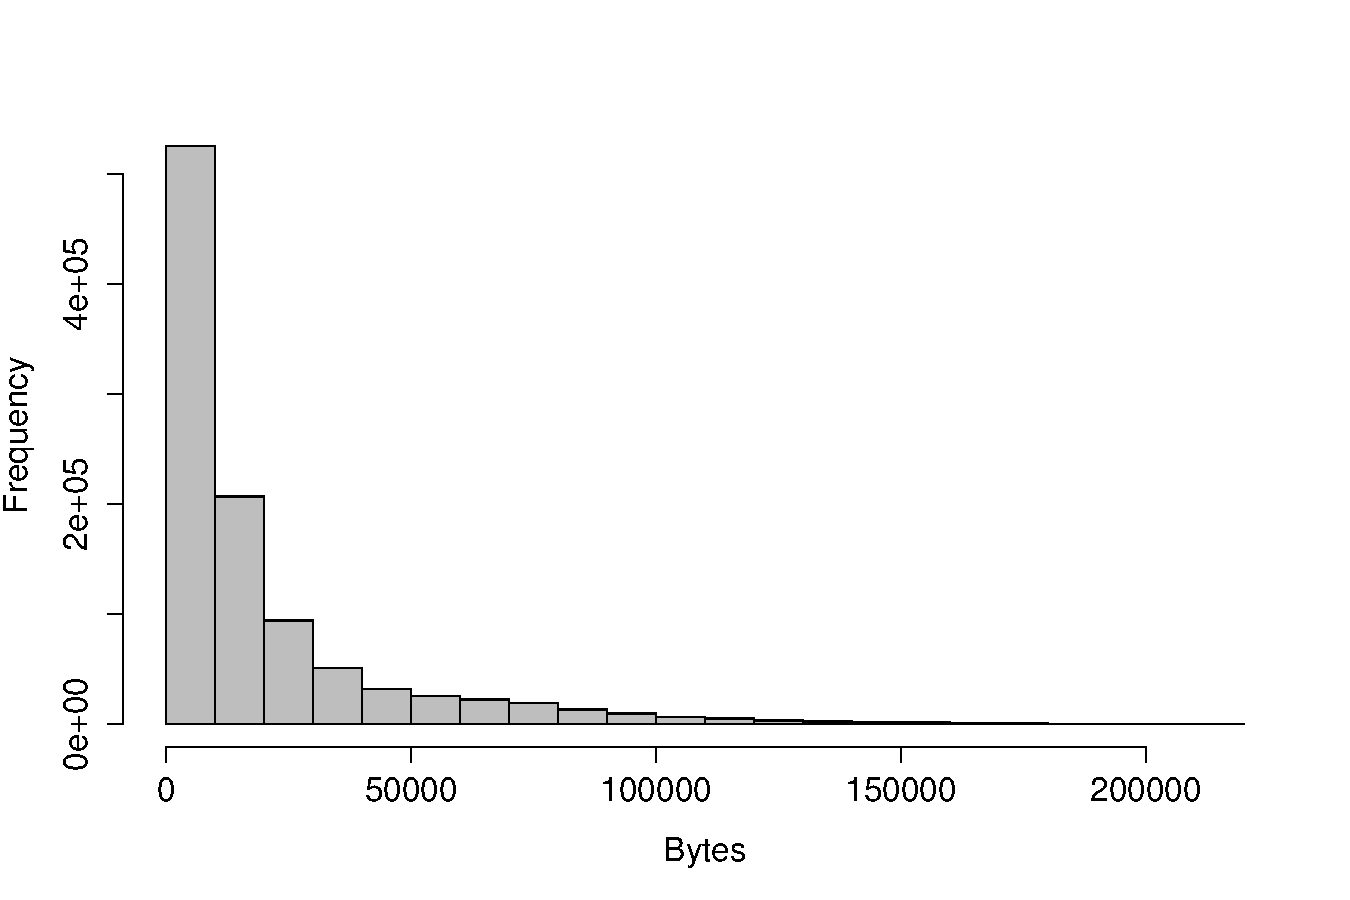
\includegraphics[width=2.2in]{figures/size-hist-NEXRAD30602.pdf}
        %\includegraphics[width=3.5in]{figures/CONDUIT_Size.eps}
        \caption{Whole size range}
        \label{NEXRAD3_Size_Whole}
    \end{subfigure}\hfill
    \begin{subfigure}{0.5\linewidth}
	\centering
    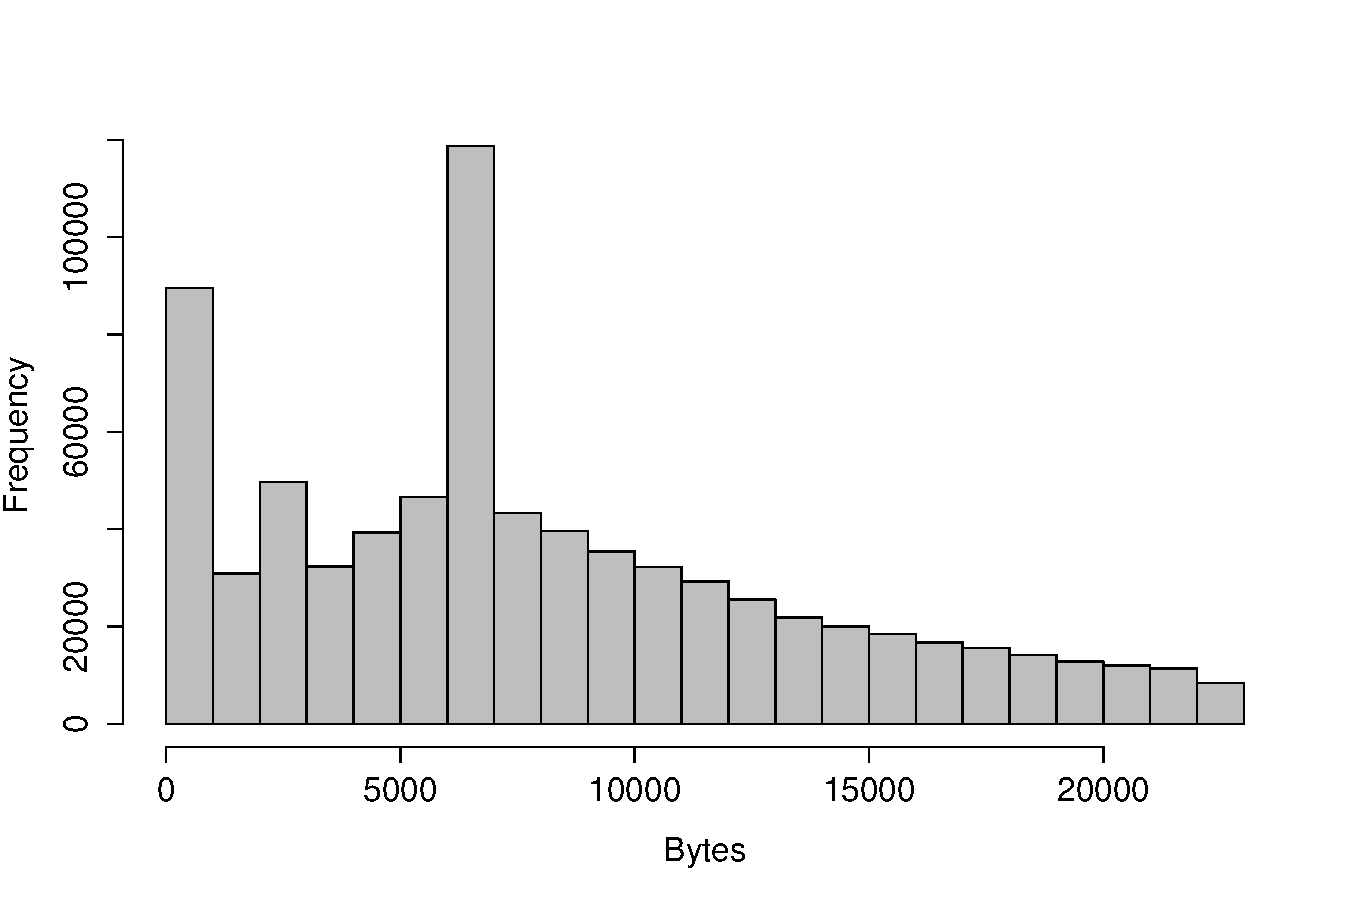
\includegraphics[width=2.2in]{figures/size-hist-NEXRAD30602-TOP75.pdf}
    %\includegraphics[width=3.5in]{figures/CONDUIT-size-75.eps}
        \caption{Top 75 percentile of size range}
        \label{NEXRAD3_Size_75}
    \end{subfigure}\hfill
    \caption{NEXRAD3 feedtype, histogram of size of data products sent on June 02, 2014}
    \label{NEXRAD3_Size}
\end{figure}

NEXRAD3 \cite{NEXRAD3} feedtype is NEXRAD level III data. Fig.~\ref{NEXRAD3_Size} indicates that the pattern of this feedtype is similar to NEXRAD2. Its file size is big with an average of 7 KB.

\begin{figure}[htb!]
\centering
    \begin{subfigure}{0.5\linewidth}
        \centering
        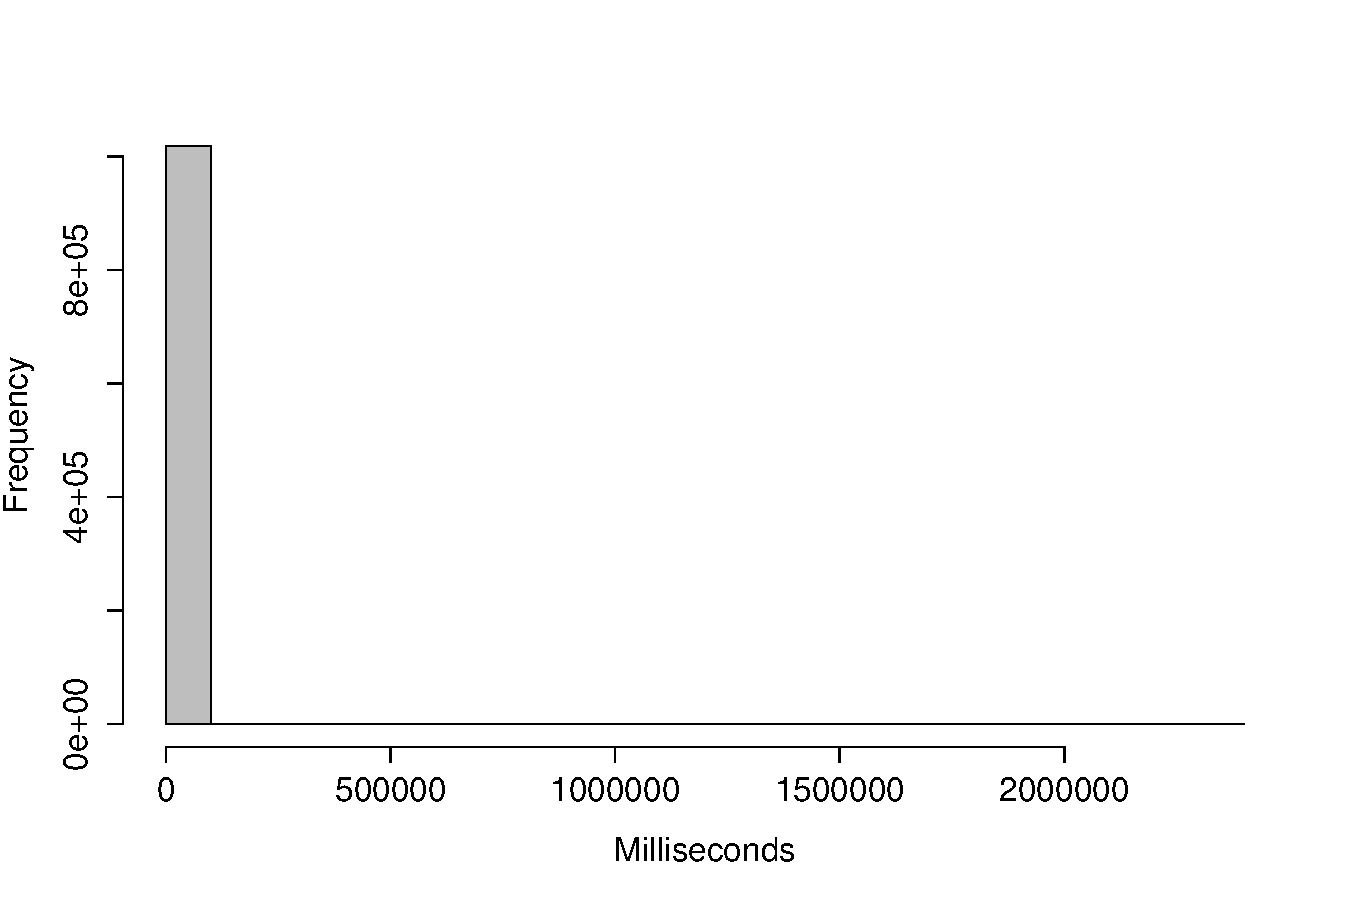
\includegraphics[width=2.2in]{figures/Inter-hist-NEXRAD30602.pdf}
        %\includegraphics[width=3.5in]{figures/CONDUIT_Size.eps}
        \caption{Whole inter-arrival time range}
        \label{NEXRAD3_Inter_Whole}
    \end{subfigure}\hfill
    \begin{subfigure}{0.5\linewidth}
	\centering
    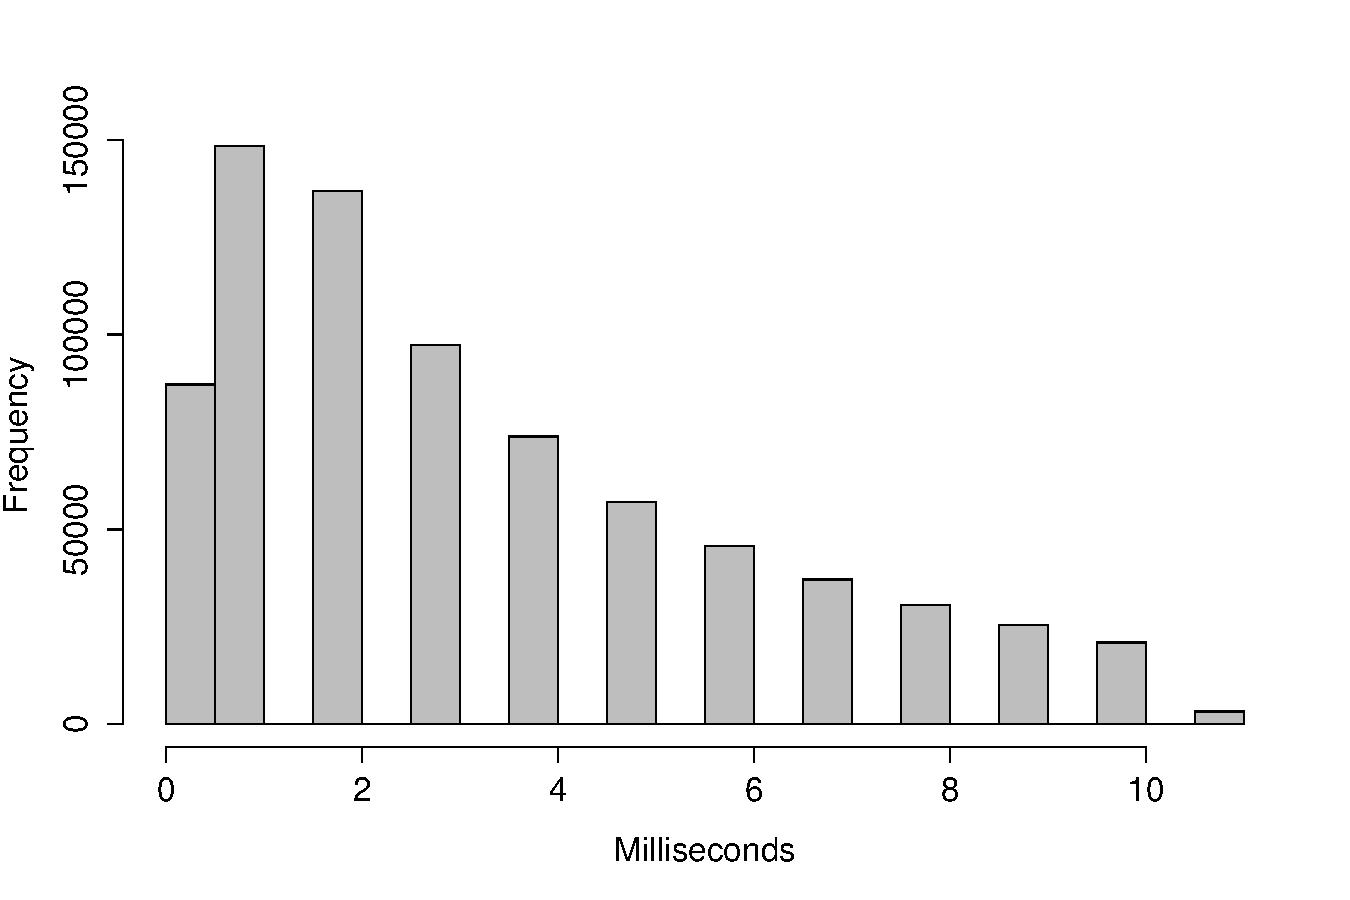
\includegraphics[width=2.2in]{figures/Inter-hist-NEXRAD30602-TOP75.pdf}
    %\includegraphics[width=3.5in]{figures/CONDUIT-size-75.eps}
        \caption{Top 75 percentile of inter-arrival time range}
        \label{NEXRAD3_Inter_75}
    \end{subfigure}\hfill
    \caption{NEXRAD3 feedtype, histograms of inter-arrival time of data products sent on June 02, 2014}
    \label{NEXRAD3_time}
\end{figure}

Fig.~\ref{NEXRAD3_time} shows that the inter-arrival time of NEXRAD3 is small, which means NEXRAD3 data products are distributed with a high frequency. The top 75\% inter-arrival time histogram Fig.~\ref{NEXRAD3_Inter_75} shows most of the data arrive within 10 millisecond after the previous one.

%FSL2
\begin{figure}[htb!]
\centering
    \begin{subfigure}{0.5\linewidth}
        \centering
        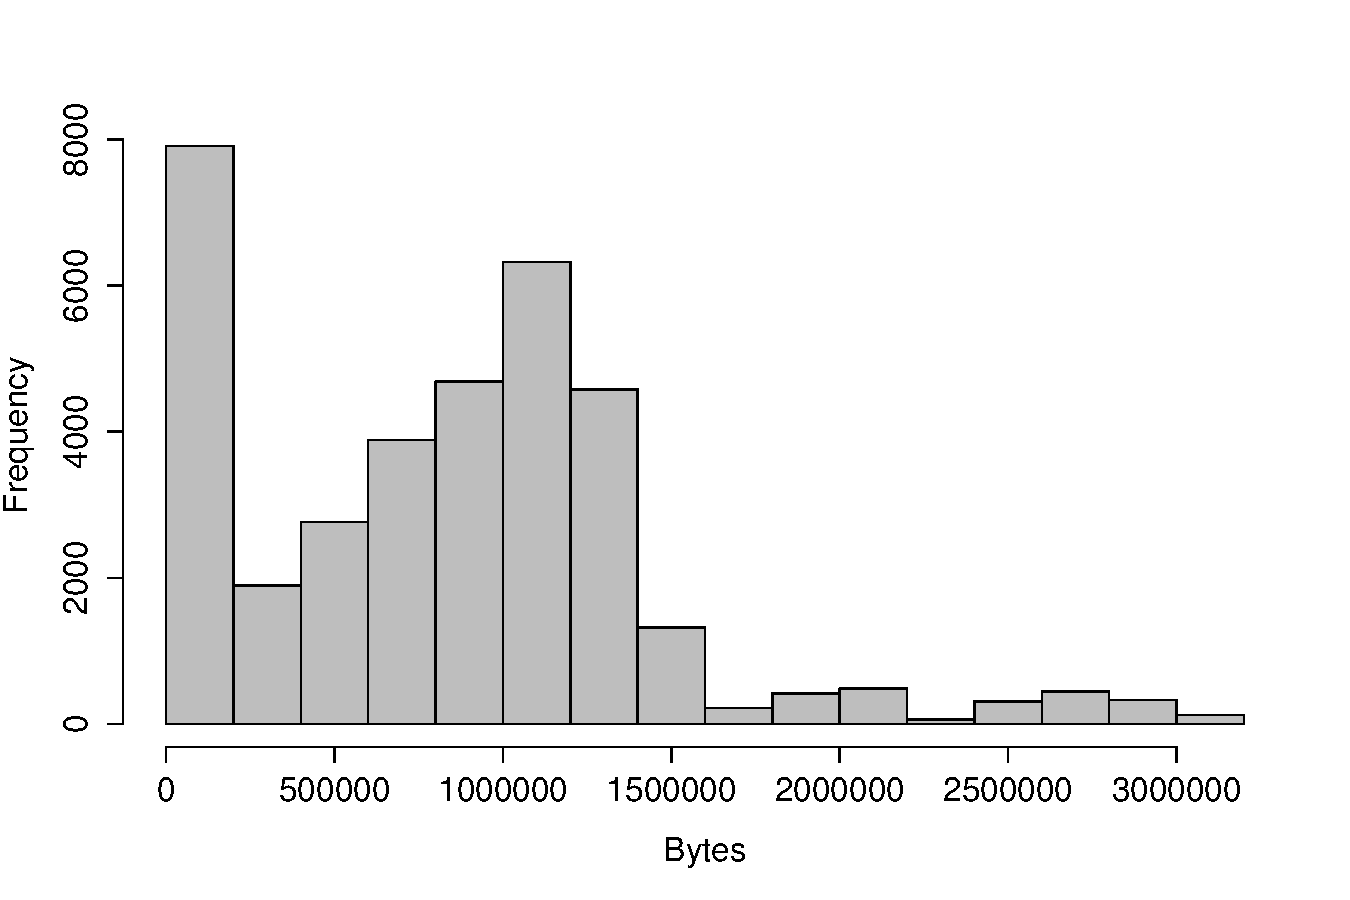
\includegraphics[width=2.2in]{figures/size-hist-FSL20602.pdf}
        %\includegraphics[width=3.5in]{figures/CONDUIT_Size.eps}
        \caption{Whole size range}
        \label{FSL2_Size_Whole}
    \end{subfigure}\hfill
    \begin{subfigure}{0.5\linewidth}
	\centering
    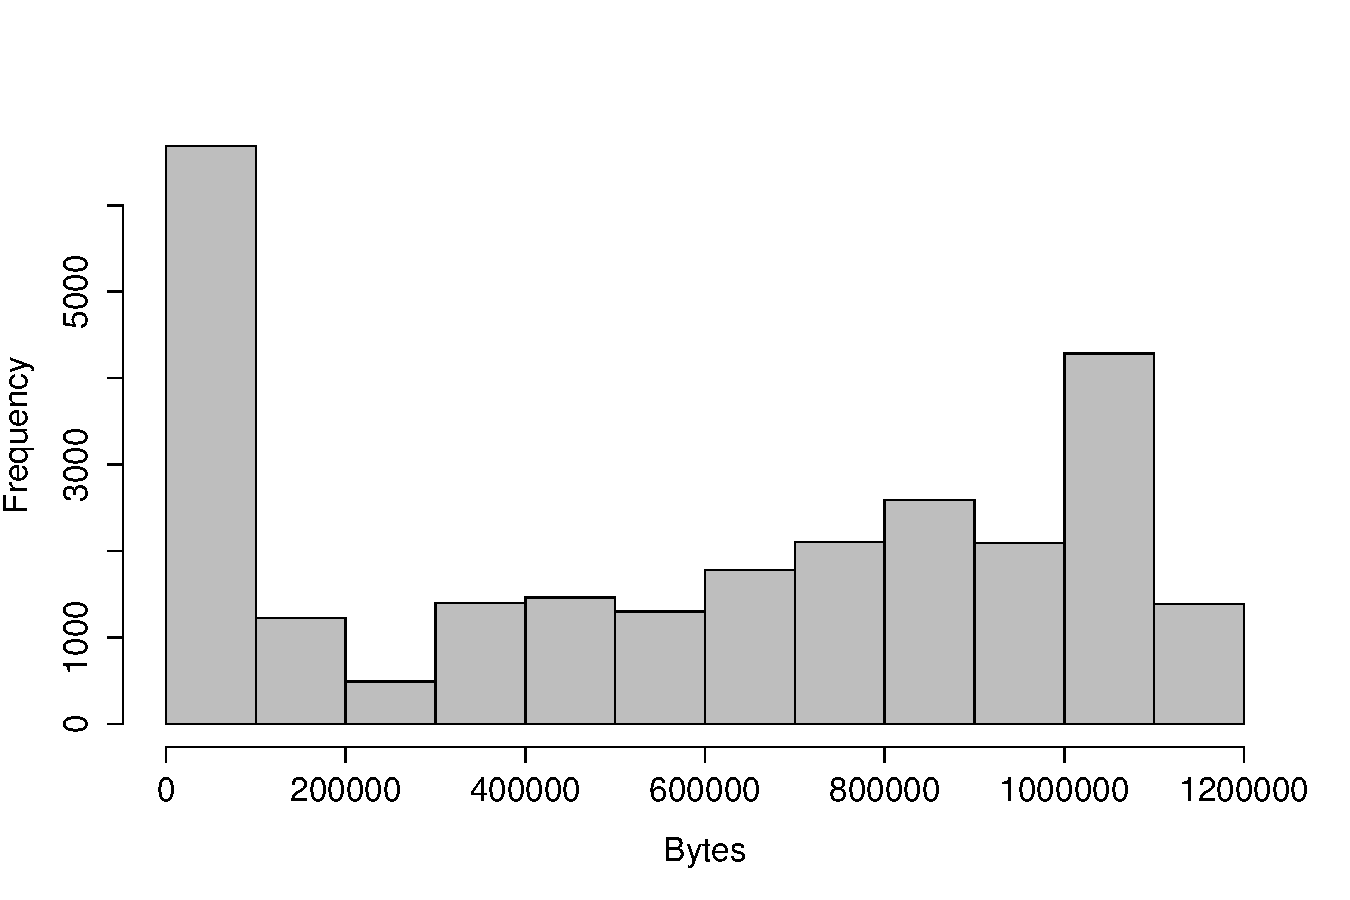
\includegraphics[width=2.2in]{figures/size-hist-FSL20602-TOP75.pdf}
    %\includegraphics[width=3.5in]{figures/CONDUIT-size-75.eps}
        \caption{Top 75 percentile of size range }
        \label{FSL2_Size_75}
    \end{subfigure}\hfill
    \caption{FSL2 feedtype, histogram of size of data products sent on June 02, 2014}
    \label{FSL2_Size}
\end{figure}

FSL2 feedtype \cite{FSL2} is NOAA Profiler Network-Forecast Systems Laboratory data, which is wind profiler data. Fig.~\ref{FSL2_Size} shows that the data size is large, usually 1MB for each data product.

\begin{figure}[htb!]
\centering
    \begin{subfigure}{0.5\linewidth}
        \centering
        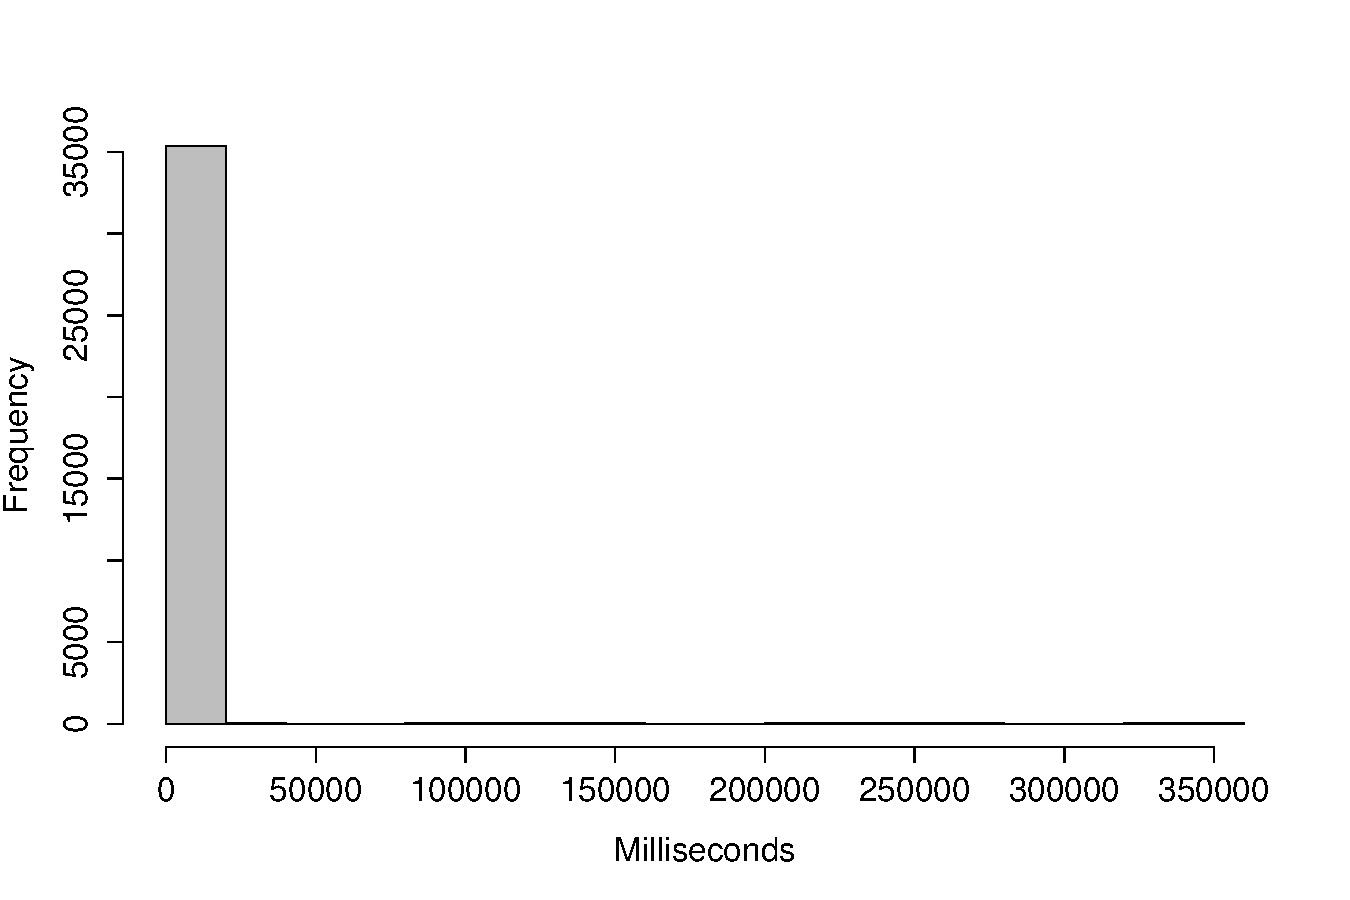
\includegraphics[width=2.2in]{figures/Inter-hist-FSL20602.pdf}
        %\includegraphics[width=3.5in]{figures/CONDUIT_Size.eps}
        \caption{Whole inter-arrival time range }
        \label{FSL2_Inter_Whole}
    \end{subfigure}\hfill
    \begin{subfigure}{0.5\linewidth}
	\centering
    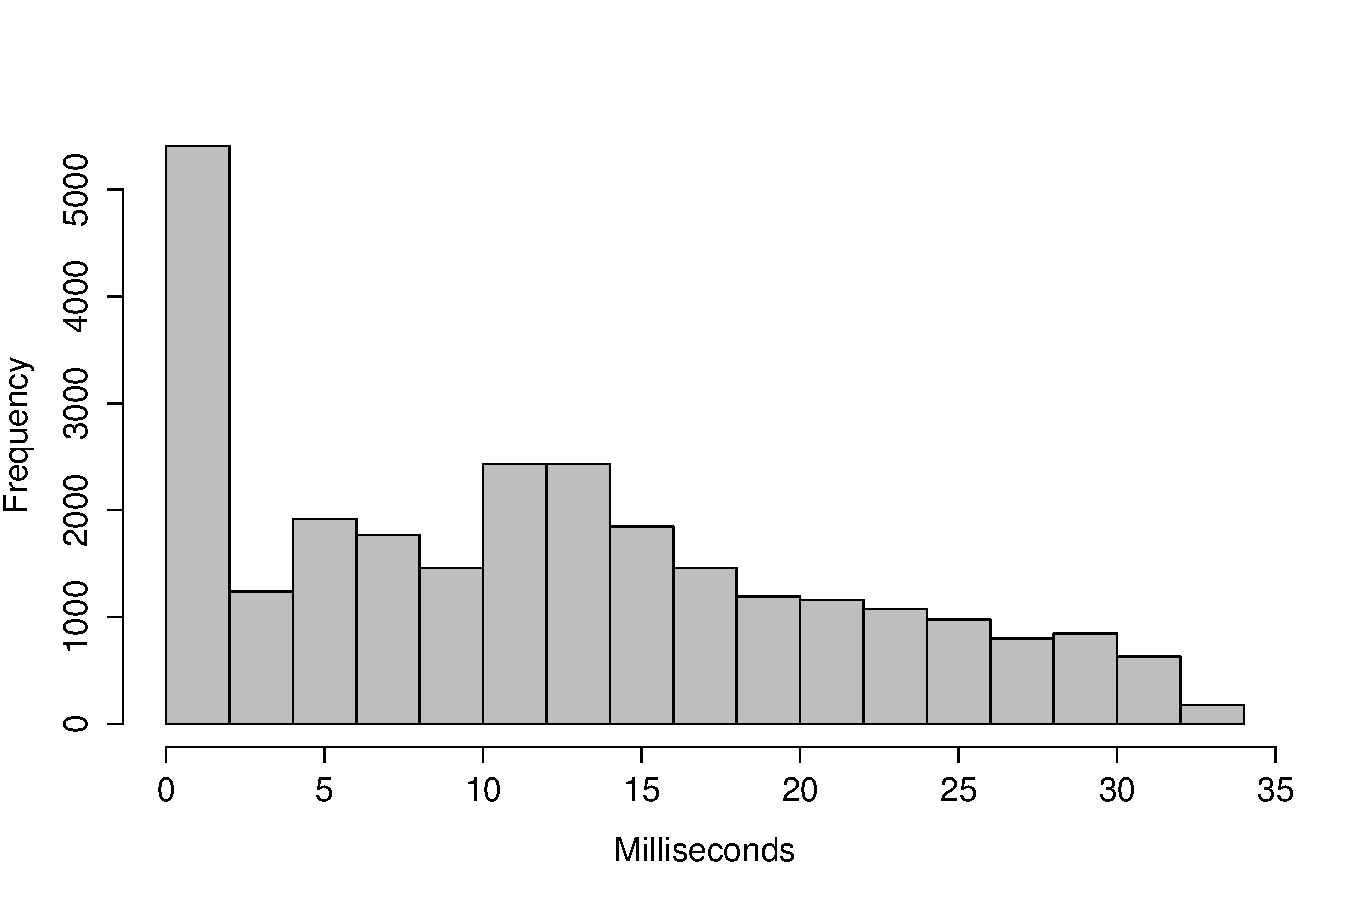
\includegraphics[width=2.2in]{figures/Inter-hist-FSL20602-TOP75.pdf}
    %\includegraphics[width=3.5in]{figures/CONDUIT-size-75.eps}
        \caption{Top 75 percentile of inter-arrival time range  }
        \label{FSL2_Inter_75}
    \end{subfigure}\hfill
    \caption{FSL2 feedtype, histogram of inter-arrival time of data products sent on June 02, 2014}
    \label{FSL2_time}
\end{figure}


\begin{figure}[htb!]
\centering
    \begin{subfigure}{0.5\linewidth}
        \centering
        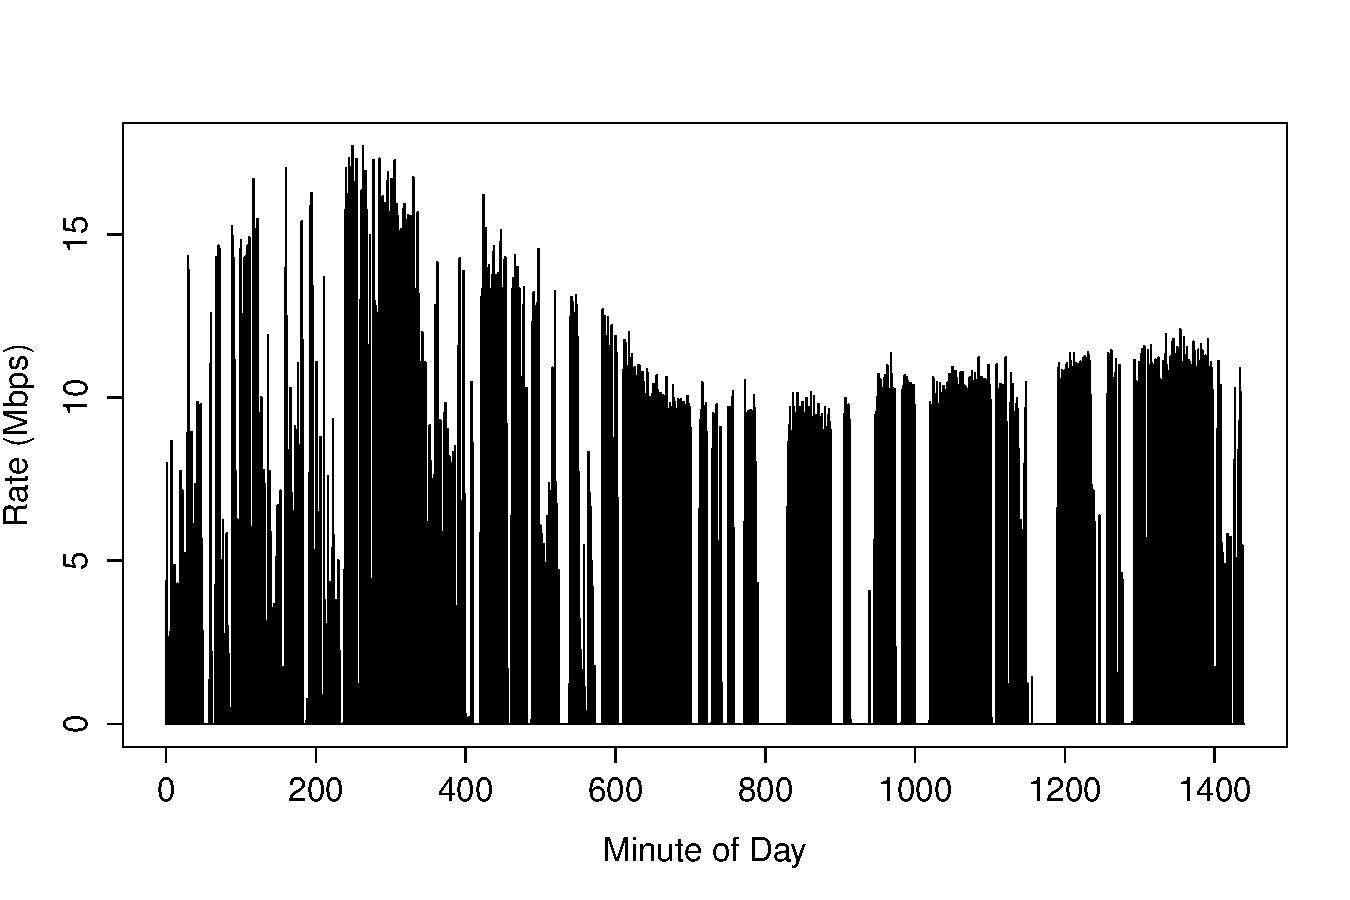
\includegraphics[width=2.2in]{figures/rate_time_NEXRAD20602.pdf}
        %\includegraphics[width=3.5in]{figures/CONDUIT_Size.eps}
        \caption{NEXRAD2 feedtype}
        \label{fig:N2-rate}
    \end{subfigure}\hfill
    \begin{subfigure}{0.5\linewidth}
	\centering
    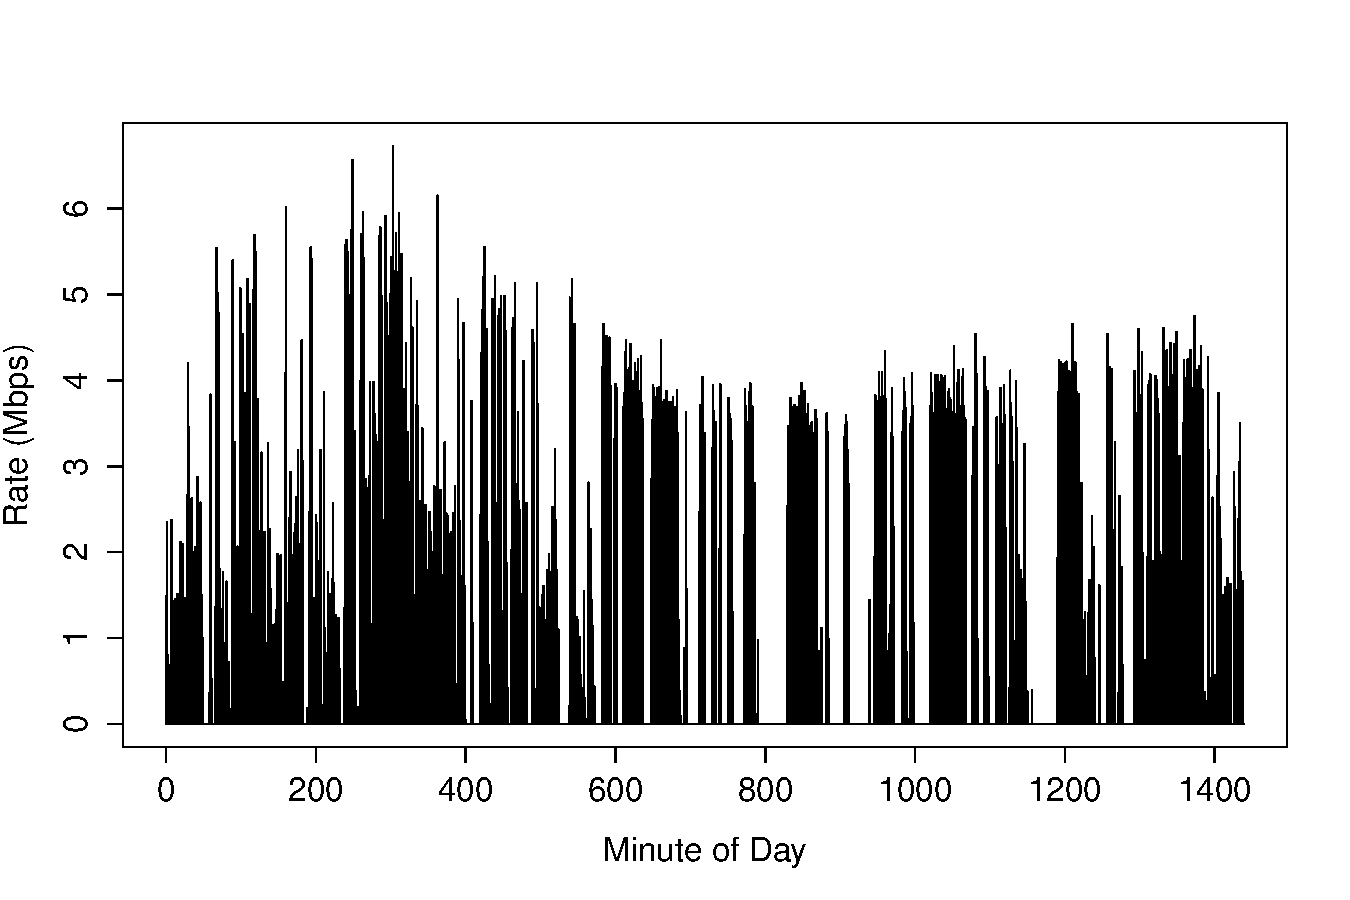
\includegraphics[width=2.2in]{figures/rate_time_NEXRAD30602.pdf}
    %\includegraphics[width=3.5in]{figures/CONDUIT-size-75.eps}
        \caption{NEXRAD3 feedtype}
        \label{fig:N3-rate}
    \end{subfigure}\hfill
    \caption{Rate vs. time of NEXRAD2 and NEXRAD3 feedtypes}
    \label{NEXRAD-rate}
\end{figure}

Fig.~\ref{NEXRAD-rate} shows that the data products arrival pattern of NEXRAD2 is similar to the pattern of NEXRAD3, but the arrival rate of NEXRAD2 is higher than that of NEXRAD3. Both NEXRAD2 and NEXRAD3 feedtypes have high throughput. 


\begin{figure}[htb!]
\centering
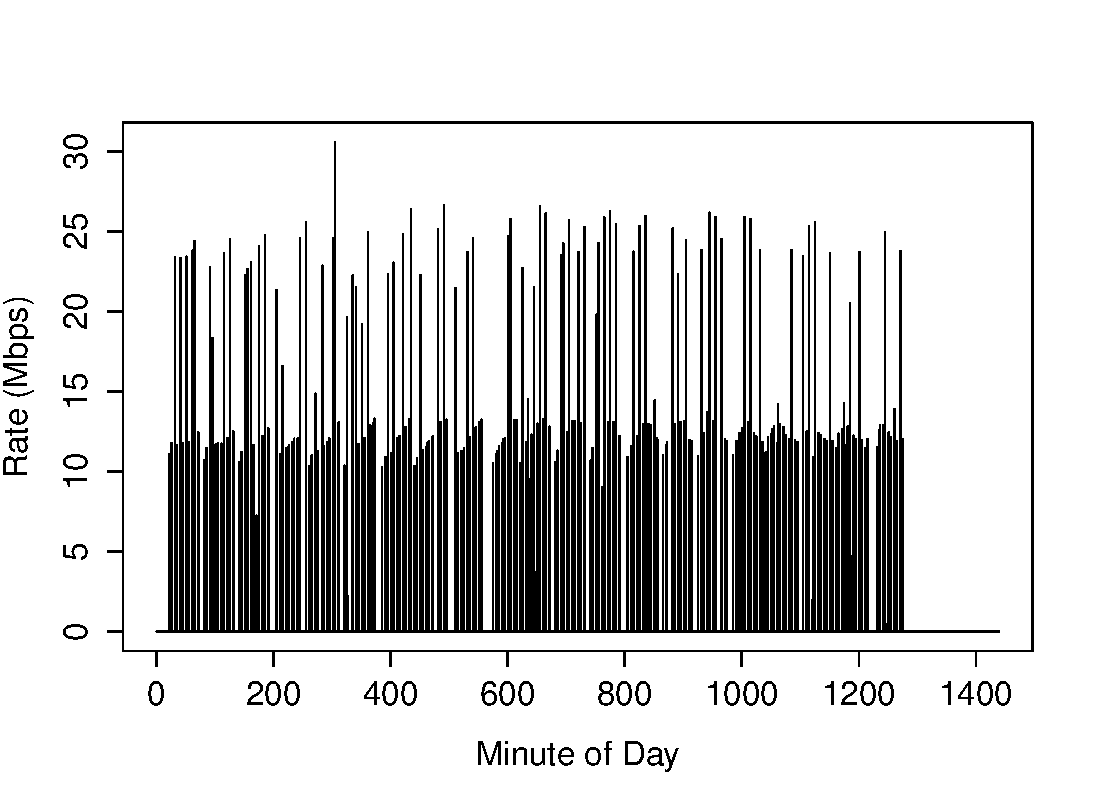
\includegraphics[width=2.2in]{figures/rate_time_FSL20602.pdf}
\caption{FSL2 feedtype}
\label{fig:FSL2-rate}
\end{figure}

Fig.~\ref{fig:FSL2-rate} shows that FSL2 feedtype consists of big-size files. It also indicates that the FSL2 data arrival rate has a periodicity about 1 hour.

% \section{Rate prediction method for SDN software}

% Follow the software guidance, software architecture graph,  

% For each program,
% Describe the language in which the program was written.
% Give name of program. State what input file the program is reading. What is the main purpose of the program? What output file is it creating?


%\section{LDM performance measurement software}


